% !TeX spellcheck = sl_SI
\documentclass[mat1]{fmfdelo}
% \documentclass[fin1]{fmfdelo}
% \documentclass[isrm1]{fmfdelo}
% \documentclass[mat2]{fmfdelo}
% \documentclass[fin2]{fmfdelo}
% \documentclass[isrm2]{fmfdelo}

% naslednje ukaze ustrezno napolnite
\avtor{Tadej Petrič}
\naslov{ZX-račun}
\title{ZX-calculus}

% navedite ime mentorja s polnim nazivom: doc.~dr.~Ime Priimek,
% izr.~prof.~dr.~Ime Priimek, prof.~dr.~Ime Priimek
% uporabite le tisti ukaz/ukaze, ki je/so za vas ustrezni
\mentor{doc.~dr.~Matija Pretnar}
%\mentorica{izr.~prof.~dr.~Ime Priimek}
%\somentor{doc.~dr.~Ime Priimek}
%\somentorica{doc.~dr.~Ime Priimek}
% \mentorja{}{}
% \mentorici{}{}

\letnica{2021} % leto diplome

%  V povzetku na kratko opišite vsebinske rezultate dela. Sem ne sodi razlaga organizacije dela --
%  v katerem poglavju/razdelku je kaj, pač pa le opis vsebine.
\povzetek{ZX-račun je nov pristop k formalizaciji kvantnega računalništva. Kvantna vezja in procese predstavimo kot barvne grafe z dodatnimi pravili za poenostavljanje, kar omogoči opis vsakega kvantnega vezja. Ogledamo si tudi različne delce ZX računa, ki omogočijo predstavitev različnih modelov kvantnega računalništva. Graf lahko pretvorimo tudi v matriko. Prikažemo tudi nekaj uporab, na primer kvantna teleportacija in kvantno iskanje.}

%  Prevod slovenskega povzetka v angleščino.
\abstract{ZX-calculus is a new approach to the formalization of quantum computing. Quantum circuits are represented with coloured graphs with added simplification rules. Using ZX-calculus, we can describe any quantum circuit. We also explore several fragments of ZX calculus and their use in describing different computational models. The graphs can also be converted to matrices. We also show a few applications, such as the quantum search algorithm and quantum teleportation.}

% navedite vsaj eno klasifikacijsko oznako --
% dostopne so na www.ams.org/mathscinet/msc/msc2010.html
\klasifikacija{81P68}
\kljucnebesede{Kvantno računalništvo, ZX-račun, graf, kategorična kvantna mehanika} % navedite nekaj ključnih pojmov, ki nastopajo v delu
\keywords{Quantum computing, ZX-calculus, graph, categorical quantum mechanics} % angleški prevod ključnih besed

\zapisiMetaPodatke  % poskrbi za metapodatke in veljaven PDF/A-1b standard

% aktivirajte pakete, ki jih potrebujete
\usepackage{tikz}
\usepackage{physics}
\usepackage{mathtools}
\usepackage{csquotes}
\usepackage{biblatex}
\usepackage{tikz}
\usepackage{quantikz}
\usepackage{amsmath}
\usepackage{graphicx}
\usepackage{stmaryrd}
%\usepackage{circuitikz}

\addbibresource{sources.bib}

% za številske množice uporabite naslednje simbole
\newcommand{\R}{\mathbb R}
\newcommand{\N}{\mathbb N}
\newcommand{\Z}{\mathbb Z}
\newcommand{\C}{\mathbb C}
\newcommand{\Q}{\mathbb Q}
\newcommand{\Hb}{\mathbb H}
\newcommand{\interpret}[1]{\left\llbracket #1 \right\rrbracket}
\DeclareMathOperator*{\im}{im}
\DeclareMathOperator*{\id}{id}
\DeclareMathOperator*{\ann}{Ann}
\DeclareMathOperator*{\spec}{Spec}

\newcommand{\E}{\mathrm{E}}
\newcommand{\Var}{\mathrm{Var}}
\newcommand{\Cov}{\mathrm{Cov}}
\newcommand{\Bias}{\mathrm{Bias}}
\renewcommand{\phi}{\varphi}
% matematične operatorje deklarirajte kot take, da jih bo Latex pravilno stavil
% \DeclareMathOperator{\conv}{conv}
% na razpolago so naslednja matematična okolja, ki jih kličemo s parom
% \begin{imeokolja}[morebitni komentar v oklepaju] ... \end{imeokolja}
%
% definicija, opomba, primer, zgled, lema, trditev, izrek, posledica, dokaz
%
\usetikzlibrary{arrows,shapes.gates.logic.US,shapes.gates.logic.IEC,calc}
\definecolor{zx_red}{RGB}{232, 165, 165}
\definecolor{zx_green}{RGB}{216, 248, 216}
\definecolor{had_yellow}{RGB}{221, 218, 28}

\tikzstyle{gn}=[circle,rounded corners=0.8em,fill=zx_green,draw=black,
  line width=0.8 pt,inner sep=3pt,minimum width=1.5em,minimum height=1.5em]
\tikzstyle{rn}=[circle,rounded corners=0.8em,fill=zx_red,draw=black,
  line width=0.8 pt,inner sep=3pt,minimum width=1.5em,minimum height=1.5em]
\tikzstyle{had}=[rectangle,fill=had_yellow,draw=black,
  line width=0.8 pt,inner sep=3pt,minimum width=1.5em,minimum height=1.5em]
\tikzstyle{none}=[]
\makeatletter
\DeclareRobustCommand{\rvdots}{%
  \vbox{
    \baselineskip4\p@\lineskiplimit\z@
    \kern-\p@
    \hbox{.}\hbox{.}\hbox{.}
  }}
\makeatother


% vstavite svoje definicije ...
%  \newcommand{}{}
\newcommand{\defeq}{\vcentcolon=}
\newcommand{\sep}{\ensuremath{.\,}}
\newcommand{\exv}{\langle}
\begin{document}

\section{Uvod}
Koncept kvantnega računalništva se je začel leta 1981, ko je Richard Feynman predlagal, kako bi lahko simulirali določene fizikalne procese z uporabo nekaterih lastnosti kvantne mehanike\cite{feynmann}. Klasični algoritmi imajo namreč težavo, da je časovna zahtevnost simulacije eksponentna glede na njeno velikost. Ker pa je narava teh simulacij pogosto probabilistična lahko uporabimo prednosti kvantne mehanike, ki je tudi sama probabilistična, da jih simuliramo bolj učinkovito, na primer z linearno kompleksnostjo. Na začetku so bili najbolj zanimivi procesi, kjer je potrebno upoštevati kvantno mehaniko -- Feynman je namreč predlagal, da so vsi kvantni sistemi na nek način ekvivalentni. Potem je simulacija preprosta, saj le izvajamo iste korake v kvantnem računalniku, kot se bi izvajali v dejanskem ekspirimentu, za rezultat pa pogledamo končno stanje računalnika.

Izkazalo pa se je, da imajo kvantni računalniki mnogo uporabe tudi izven fizikalnih simulacij: Shorov algoritem sprejme število, in vrne njegove prafaktorje. Ta problem je klasično zelo težek, ne vemo še, ali obstaja učinkovita rešitev, kvantno pa poznamo rešitev, ki deluje hitreje kot eksponentno. Podobno obstaja mnogo drugih težkih problemov za katere imamo hitro kvantno rešitev, na primer iskanje inverzne funkcije, Fourierjeva transformacija, iskanje diskretnega logaritma...

Pomembno vprašanje je kako formalizirati kvantne računalnike in kako jih programirati. John Von Neumann je formaliziral kvantno mehaniko z uporabo Hilbertih prostorov, ta pristop je najbolj pogosto uporabljen še danes\cite{neumann}. Izkaže pa se, da velik del teorije postane bolj naraven, če uporabimo drugačen pristop. To je kmalu predlagal že Neumann z kvantno logiko, vendar se pristop takrat še ni uveljavil, kar je močno obžaloval. Iz kvantne logike se je razvil moderni pristop, kategorična kvantna mehanika. Tukaj lahko mnoge zakone opišemo le z diagrami, kar naredi mnogo dejstev bolj naravnih, ne izgubimo pa nič natančnosti. Iz kategorične kvantne mehanike se je razvil ZX-račun, ki ga uporabljamo za opis kvantnih vrat in vezij z uporabo diagramov. Znotraj samega ZX-računa pa bo marsikaj bolj enostavno, na primer iskanje algoritmov, iskanje novih fizikalnih zakonov in poenostavljanje vezij.

\section{Klasično računalništvo}
Za opis kvantnega računalništva je koristno najprej poznati delovanje klasičnih računalnikov. 
\subsection{Biti in vrata}
Klasični računalniki so zgrajeni na osnovi Boolove algebre. Osnovni objekti so biti, imajo lahko vrednosti \(0\) in \(1\), ustrezajo pa logični neresnici in logični resnici. Namesto \(1\) bomo uporabljali \(\ket{1}\), namesto \(0\) pa pišemo \(\ket{0}\), saj nam to olajša prehod na kvantne računalnike, prav tako pa jih težje zamenjamo z naravnima številoma \(0\) in \(1\). Naredimo množico bitov \(B = \{\ket0, \ket1\}\).

Bite lahko združimo v skupine. Skupina bitov je element kartezičnega produkta množice bitov. Kot primer, skupina treh bitov je \(B^3\), primer elementa te skupine pa je \((\ket0, \ket1, \ket0)\). Uvedemo preprostejši zapis za skupine: 
\begin{align*}
    \ket{a} \defeq& (\ket a)\\
    \ket{ab} \defeq& (\ket{a},\ket b)\\
    \ket{abc} \defeq& (\ket a, \ket b, \ket c)\\
    &\vdots
\end{align*}

Funkcije skupin bitov imenujemo logična vrata oziroma. Najbolj osnovna vrata so vrata za konjunkcijo, disjunkcijo in negacijo.
\begin{align*}
    \land(\ket{ab}) = \ket{a}\land\ket{b} = \ket{a\land b},\\
    \lor(\ket{ab}) = \ket{a}\lor\ket{b} = \ket{a\lor b},\\
    \lnot\ket{a} = \ket{\lnot a}.
\end{align*}
Izkaže se, da je zgornji nabor operacij (skupaj s kompozicijo) dovolj, da izrazimo poljubno funkcijo \(B^n\to B\).
\begin{definicija}
    Množica logičnih vrat \(B^2\to B\) je funkcijsko polna, če lahko poljubno funkcijo \(B^n\to B\) predstavimo kot kompozicijo vrat iz te množice.
\end{definicija}
Izkaže se, da obstajajo še preprostejši primeri funkcijsko polnih naborov operatorjev. Najbolj znan je NAND, ki ga predstavimo kot \(\downarrow\)
\begin{align*}
    \ket{a}\downarrow \ket{b} = \lnot (\ket{a} \land \ket{b}),
\end{align*}
obstajajo pa še ostali, kot naprimer NOR.\cite{sheffers}

Pogosto raje uporabljamo grafični zapis logičnih vrat. To je še posebej pomembno, saj se podobna grafična vezja definira tudi za kvantne računalnike. Začnemo z najenostavnejšimi logičnimi vrati, vrati za negacijo
\begin{center}
    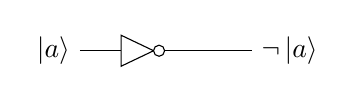
\begin{tikzpicture}
        \node[not gate US, draw, logic gate inputs=n] (neg) at (0,0){};
        \node (a) at (-1,0) {\(\ket{a}\)};
        \node (out) at (2,0) {\(\lnot \ket{a}\)};
        \draw (a) to (neg.input);
        \draw (neg.output) to (out);
    \end{tikzpicture}.
\end{center}
Na levi strani pišemo vhode (v tem primeru \(\ket{a}\)), črte pa predstavljajo kompozicijo oziroma tok podatkov. Tukaj gre bit \(\ket{a}\) v vrata za negacijo. Na desni strani vrat pa dobimo negiran bit. Takemu diagramu lahko rečemo vezje, ogledamo si še malo bolj zapleten primer. Tukaj predstavimo De Morganov zakon
\[
    \lnot(\ket{a}\land \ket{b}) = \lnot\ket{a} \lor \lnot \ket{b}
\]
\begin{center}
    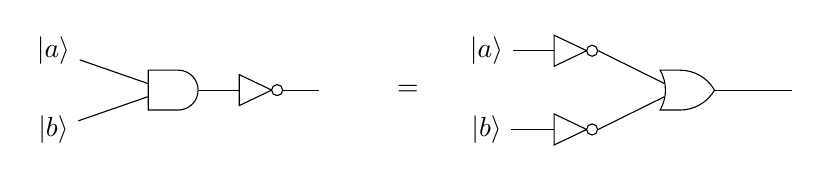
\begin{tikzpicture}
        \node[and gate US, draw, logic gate inputs=nn] (and) at (0,0){};
        \node[not gate US, draw, logic gate inputs=n] (neg) at (1,0){};
        \node (equal) at (3,0) {\(=\)};
        \node[or gate US, draw, logic gate inputs=nn] (or) at ($(equal)+(3.5,0)$){};
        \node[not gate US, draw, logic gate inputs=n] (nega) at ($(equal)+(2,0.5)$){};
        \node[not gate US, draw, logic gate inputs=n] (negb) at ($(equal)+(2,-0.5)$){};
        \node (a) at ($(equal)+(1,0.5)$) {\(\ket{a}\)};
        \node (b) at ($(equal)+(1,-0.5)$) {\(\ket{b}\)};
        \node (out) at ($(equal)+(5,0)$) {};
        \node (a1) at (-1.5,-0.5) {\(\ket{b}\)};
        \node (b1) at (-1.5,0.5) {\(\ket{a}\)};
        \node (out1) at (2,0) {};
        \draw (a1) to (and.input 2);
        \draw (b1) to (and.input 1);
        \draw (and.output) to (neg.input);
        \draw (neg.output) to (out1);
        \draw (a) to (nega.input);
        \draw (b) to (negb.input);
        \draw (or.output) to (out);
        \draw (nega.output) to (or.input 1);
        \draw (negb.output) to (or.input 2);
    \end{tikzpicture}.
\end{center}
Na levi strani imamo logična vrata za konjunkcijo, v katero vodita dva vhoda. Rezultat te operacije pa kasneje negiramo. Izhodne vrednosti ponavadi ne pišemo, saj bi bila enaka grafični predstavitvi vezja. Na desni strani enakosti pa vhode najprej negiramo, od tja pa podatke preusmerimo v vrata za disjunkcijo, iz katerih dobimo rezultat vezja. Po De Morganovem izreku sta vezji enaki.

Nazadnje si ogledamo še vrata NAND
\begin{center}
    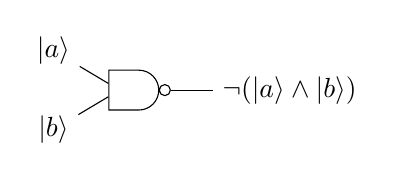
\begin{tikzpicture}
        \node[nand gate US, draw, logic gate inputs=nn] (nand) at (0,0){};
        \node (ina) at (-1, 0.5) {\(\ket{a}\)};
        \node (inb) at (-1, -0.5) {\(\ket{b}\)};
        \node (out) at (2, 0) {\(\lnot(\ket a\land \ket b)\)};
        \draw (ina) to (nand.input 1);
        \draw (inb) to (nand.input 2);
        \draw (nand.output) to (out);
    \end{tikzpicture},
\end{center}
vrata za negacijo z uporabo NAND pa bi bile
\begin{center}
    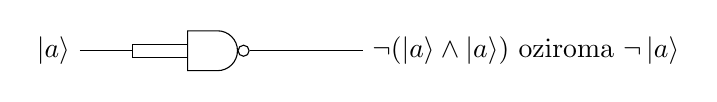
\begin{tikzpicture}
        \node[nand gate US, draw, logic gate inputs=nn] (nand) at (0,0){};
        \node (ina) at (-2, 0) {\(\ket{a}\)};
        \node (brunch) at (-1,0) {};
        \node (out) at (4, 0) {\(\lnot(\ket a\land \ket a)\) oziroma \(\lnot \ket{a}\)};
        \draw (ina) -- (-1,0) |- (nand.input 1);
        \draw (ina) -- (-1,0) |- (nand.input 2);
        \draw (nand.output) to (out);
    \end{tikzpicture}.
\end{center}
S pomočjo vrat za negacijo lahko enostavno izrazimo vrata za konjunkcijo, z De Morganovim zakonom pa tudi za disjunkcijo. Tako kmalu vidimo, da lahko poljubno vezje predstavimo le z vrati NAND.

\subsection{Implementacija}
Glavni razlog, za grafični zapis vezij je podobnost z realno implementacijo v elektronskih vezjih. Logična vrata so enostavno dostopna, ponavadi implementirana z tranzistorji, povezave med njimi pa predstavljajo žice. Logične vrednosti predstavimo z električno napetostjo. Tako lahko za logično vrednost \(1\) uporabimo \(+5\)V (pogosta je tudi vrednost \(+3.3\)V), za \(0\) pa uporabimo \(0\)V.
\subsection{Klasična komunikacija}

%----------------------------------------------------------- KONEC KLASIČNO ------------------------------------------------------------------------------

\section{Kvantna mehanika}
Klasični pristop do kvantne mehanike uporablja Hilbertove prostore\cite[stran 12]{mathforqm}.

\begin{definicija} \(\Hb\) je Hilbertov prostor če je vektorski prostor s skalarnim produktom
    \begin{align*}
        \braket{\cdot}{\cdot} :& \Hb \times \Hb \to \C\\
        & (\psi, \varphi) \mapsto \braket{\varphi}{\psi},
    \end{align*}
    za katerega za vse \(\phi, \varphi, \varphi_1, \varphi_2 \in \Hb\) velja
    \begin{align*}
        \braket{\psi}{\varphi} &= \overline{\braket{\varphi}{\psi}},\\
        \braket\psi &\geq 0,\\
        \braket\psi = 0 &\iff \psi = 0,\\
        \forall a,b\in\C\sep \braket{\psi}{a\varphi_1 + b\varphi_2} &=a\braket{\psi}{\varphi_1} + b\braket{\psi}{\varphi_2}.
    \end{align*}
    Ta skalarni produkt pa inducira normo
    \begin{align*}
        \norm*{\cdot} : \Hb &\to \R\\
        \psi &\mapsto \sqrt{\braket\psi},
    \end{align*}
    v katerem je \(\Hb\) poln.
\end{definicija}

Linearne preslikave \(\Hb\to\Hb\) so operatorji. Če je \(\forall \psi,\phi\in\Hb\sep\braket{A^*\psi}{\varphi} = \braket{\psi}{A\varphi}\) je \(A^*\) adjungirani operator operatorja \(A\). Operator \(U\) je unitaren če \(\forall \psi,\varphi\in\Hb\sep \braket{U\psi}{U\varphi} = \braket{\psi}{\varphi}\).

Vektorje bomo pisali v Diracovem zapisu. Elementi \(\Hb\) so tako \(\ket{\psi}\in\Hb\), temu rečemo ket. Znotraj skalarnih produktov ketov ponavadi ne pišemo, tako dobimo \(\braket{\ket\psi}{\ket\varphi} = \braket{\psi}{\varphi}\). Elementi dualnega prostora pa so braji:
\begin{align*}
    \bra{\psi} \defeq \left(\varphi \mapsto \braket{\psi}{\varphi} \right).
\end{align*}
Tukaj opazimo, da velja \(\bra{\psi}\, \ket{\varphi} = \braket{\psi}{\varphi}\).

Pomembni so še lastni vektorji in projekcije: \(\ket{\psi}\) je lastni vektor za \(A\) z lastno vrednostjo \(\lambda\), če \(A\ket\psi = \lambda \ket\psi\); \(P\) je projekcija, če \(P^2 = P\). Če je poleg tega še \(P^* = P\) je projekcija ortogonalna.

Za sestavljanje novih Hilbertovih prostorov iz starih nam bo služil tenzorski produkt. Ta nam bo omogočil, da združimo opis dveh kvantnih delcev v en sam sistem. Najprej definiramo tenzorski produkt kot preslikava
\begin{align*}
    \ket\varphi \otimes \ket\psi : \Hb_1 \times \Hb_2 &\to \mathbb C\\
    (u,v) &\mapsto \braket{u}{\varphi}_1 \braket{v}{\psi}_2.
\end{align*}
Linearna ogrinjača takih vektorjev sestavi vektorski prostor \(\Hb_1 \otimes \Hb_2\). Tenzorski produkt večih prostorov naredimo induktivno, najprej tenzorski produkt prvih dveh, dobljenega tenzorsko množimo s tretjim in tako naprej. Prav tako za elemente. Za to nam bo prav prišla oznaka
\begin{align*}
    \ket{\varphi}^{\otimes n} = \bigotimes_{j=1}^n \ket\varphi.
\end{align*}
\subsection{Von Neumannova slika}
\subsubsection{Kvantna stanja in opazljivke}
Kvantna stanja so elementi Hilbertovega prostora \(\ket\psi\in\Hb\), za katere velja \(\norm{\ket\psi} = 1\). Opazljivka je merljiva količina kvantnega sistema (na primer hitrost ali pozicija). Predstavimo jo z sebi-adjungiranim operatorjem \(\Hb\). Definiramo oznako
\begin{align*}
    \ev{A}_\psi = \braket{\psi}{A\psi},
\end{align*}
ki jo imenujemo pričakovana vrednost opazljivke \(A\) v stanju \(\ket\psi\).
\subsubsection{Meritve}
V kvantnih sistemih lahko izmerimo opazljivke. Možni rezultati meritev so točno lastne vrednosti operatorja, ki predstavlja opazljivko. Rečemo da je verjetnost \(P_\psi(\lambda)\), da za kvantni sistem, ki je v stanju \(\ket\psi\) dobimo po meritvi opazljivke \(A\) lastno vrednost \(\lambda\) točno 
\begin{align*}
    P_\psi(\lambda) = \norm{P_\lambda \ket\psi}^2,
\end{align*}
kjer je \(P_\lambda\) projekcija na lastni podprostor z lastno vrednostjo \(\lambda\).
\subsubsection{Spin}
Spin je lastnost osnovnih delcov, podobno kot recimo njihova masa. Fizikalno je spin navidezno vrtenje delcev: imajo vrtilno količino ampak se ne vrtijo. Za osnovne delce bi bilo dejansko vrtenje celo nesmiselno, saj so delci točkasti brez volumna ali polmera. Ne glede na to pa spin še vedno lahko spin še vedno izmerimo, prav tako pa ima mnoge posledice na okolje. V kvantnem računalništvu bomo spin izrabljali za predstavitev kubitov. Da lahko vrednost spina spremljamo uporabimo Paulijeve matrike.
\begin{definicija} Paulijeve matrike so \(2\times 2\) unitarne kompleksne matrike:
    \begin{align*}
        X &= \sigma_x \defeq \begin{bmatrix}
            0&1\\
            1&0
        \end{bmatrix},\\
        Y &= \sigma_y \defeq \begin{bmatrix}
            0&-i\\
            i&0
        \end{bmatrix},\\
        Z &= \sigma_z \defeq \begin{bmatrix}
            1&0\\
            0&-1
        \end{bmatrix}.
    \end{align*}
\end{definicija}
Opazljivke spina dobimo, če Paulijeve matrike delimo z \(2\). Te imajo lastne vrednosti \(\pm \frac12\) in jih uporabimo za meritve v naravi. V navadi pa je, da faktorja \(\frac12\) ne pišemo in kot opazljivke uporabimo le \(\sigma_x\) in \(\sigma_z\).
\subsection{Kubiti}
Kubite definiramo kot elemente Hilbertovega prostora \(\mathbb C^2\) dolžine \(1\). Kot njihove opazljivke uporabimo paulijeve matrike. Če gledamo le spin v \(z\) smeri, uporabljamo opazljivko \(\sigma_z\), ki ima lastne vrednosti \(\{+1, -1\}\). Tem lastnim vrednostim ustrezajo lastni vektorji \(\ket0\) in \(\ket1\), ki jih definiramo kot
\begin{align*}
    \ket0 \defeq \begin{bmatrix}
        1\\0
    \end{bmatrix}\\
    \ket1 \defeq \begin{bmatrix}
        0\\1
    \end{bmatrix}
\end{align*}
Opazimo, da to sestavlja bazo vektorskega prostora. Kubit lahko tako napišemo kot linearno kombinacijo \(\ket0\) in \(\ket1\). Tukaj lahko vidimo vzporednico s klasičnim računalništvom: tam so bili biti le \(\ket0\) in \(\ket1\), tukaj pa tudi vse vrednosti vmes! Eksplicitno, poljubni kubit je oblike \(a\ket0+b\ket1\) kjer \(a^2+b^2=1\).

Definiramo si še Bellova stanja
\begin{align*}
    \ket{+} \defeq \frac{1}{\sqrt2} (\ket0+\ket1)\\
    \ket{-} \defeq \frac{1}{\sqrt2} (\ket0-\ket1).
\end{align*}
Ustrezajo lastnim vektorjem opazljivke \(\sigma_x\), ki spremlja spin v \(x\) smeri. Spina \(X\) in \(Z\) sta dualna, kar ima posledico, da ima vsak izrek o \(Z\) spinu analogno trditev o \(X\) spinu, le vse \(\ket+\) zamenjamo s \(\ket0\) in obratno, prav tako pa zamenjamo \(\ket-\) s \(\ket1\).

Podobno kot pri klasičnem računalniku potrebujemo sisteme več bitov, pri kvantnih računalnikih potrebujemo sisteme večih kubitov. Fizično ga pogosto predstavimo kot računalnik z večimi elektroni, en za vsak kubit. Tukaj uporabimo tenzorski produkt. Sistem dveh kubitov bi tako označili \(\mathbb C^2 \otimes \mathbb C^2\). Vpeljemo si še krajšo oznako za elemente:
\begin{align*}
    \ket{ab} \defeq& \ket{a}\otimes\ket{b}\\
    \ket{abc} \defeq& \ket{a}\otimes\ket{b}\otimes\ket{c}\\
    &\vdots
\end{align*}
S to oznako lahko preprosto napišemo poljuben element \(\mathbb C^2 \otimes \mathbb C^2\) kot
\begin{align*}
    a\ket{00} + b\ket{01} + c\ket{10} + d\ket{11}.
\end{align*}
Hitro opazimo, da dimenzija vektorskega prostora narašča eksponentno. Sistem dveh kubitov je dimenzije \(2^2\), sistem treh je \(2^3\), sistem \(n\) kubitov pa \(2^n\). Ta lastnost kvantnim računalnikom omogoča procesiranje velike količine podatkov z zelo malo kubiti.
\subsection{Bellov izrek}
\subsection{Kvantna vrata}
\subsection{Kvantna vezja}
\subsection{Implementacija}

%----------------------------- ZX CALC -------------------------------------------

\section{ZX-račun}
V ZX-računu vezja predstavljamo kot graf. To ima mnogo prednosti, saj so pogosto diagrami bolj pregledni ter poenostavljanje diagramov bolj preprosto. Ključno je, da lahko definiramo diagrame, ki so ekvivalentni vezjem (oziroma predstavljajo linearne preslikave), saj te ustrezajo kvantnim procesom. Potem si definiramo dovoljene operacije nad temi grafi, ki so na nek način kompatibilne z operacijami na matrikah vendar naravne ter enostavne za uporabo. Cilj pa je, da z diagrami popolnoma nadomestimo klasični pogled (z klasičnimi kvantnimi vezji in pa linearnimi preslikavami) ter, kjer je mogoče, opisujemo lastnosti le z uporabo ZX-diagramov kot osnovno orodje.
\subsection{Pajki}
Vozlišča v grafu se imenujejo pajki. Poznamo dva primarna tipa pajkov, Z pajek (barvamo zeleno) in X pajek (barvamo rdeče).
\begin{center}
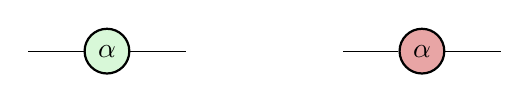
\begin{tikzpicture}
    \node [style=gn] (2) at (1,0) {\(\alpha\)};
    \node [style=rn] (1) at (5,0) {\(\alpha\)};
    \draw (0,0) to (2);
    \draw (2) to (2,0);
    \draw (4,0) to (1);
    \draw (1) to (6,0);
\end{tikzpicture}
\end{center}
Kadar je \(\alpha = 0\) faze ne pišemo, pajek ostane le zeleno ali rdeče pobarvan disk.

Lahko imata poljubno število vhodov ali izhodov. V temu članku bomo pisali vhode na levi strani, izhode pa na desni strani pajka (izkaže pa se, da to ne spremeni vezja, le pomaga intuiciji). Kot primer, Z pajek z tremi vhodi in dvema izhodoma je

\begin{center}
  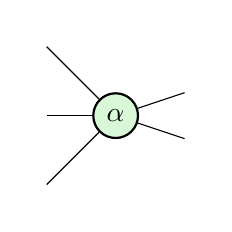
\begin{tikzpicture}
    \node (01) at (0, 0) {};
    \node (02) at (0, 1) {};
    \node (03) at (0, 2) {};
    \node [style=gn] (1) at (1.00, 1.00) {\(\alpha\)};
    \node (21) at (2, 0.66666) {};
    \node (22) at (2, 1.33333) {};
    \draw (01) to (1);
    \draw (02) to (1);
    \draw (03) to (1);
    \draw (1) to (21);
    \draw (1) to (22);
  \end{tikzpicture}.
\end{center}

Pajki ustrezajo linearnim preslikavam \cite[poglavje 1.1]{Backens}. Definiramo, da Z pajku z \(n\) vhodi in \(m\) izhodi pripada preslikava
\begin{align*}
    \ket{0}^{\otimes m} \bra{0}^{\otimes n} + e^{i\alpha}\ket{1}^{\otimes m} \bra{1}^{\otimes n}.
\end{align*}
To preslikavo lahko napišemo tudi kot \(2^n\times 2^m\) matriko. Element na mestu \((1,1)\) ustreza \(\ket{0}^{\otimes m} \bra{0}^{\otimes n}\) delu preslikave, element na mestu \((2^n, 2^m)\) pa \(\ket{1}^{\otimes m} \bra{1}^{\otimes n}\) delu preslikave. Če \((n,m)\neq (0,0)\) potem dobimo
\begin{align*}
    \begin{bmatrix}
        1 & 0 & \cdots & 0 \\
        0 & 0 & \cdots & 0 \\
        \vdots & \vdots & \ddots & 0 \\
        0 & 0 & 0 & e^{i\alpha} 
        \end{bmatrix}.
\end{align*}
Pajek brez vhodov ali izhodov z fazo \(\alpha\) pa napišemo kot skalar \(1+e^{i\alpha}\).
Podobno bi lahko definirali X pajek z \(n\) vhodi in \(m\) izhodi \cite{workingcs} kot
\begin{align*}
    \ket{+}^{\otimes m} \bra{+}^{\otimes n} + e^{i\alpha}\ket{-}^{\otimes m} \bra{-}^{\otimes n}.
\end{align*}

To lahko posplošimo in definiramo operator \(\interpret{\cdot}: (D:n\to m)\to (\interpret{D}: \C^{2^n} \to \C^{2^m})\), ki poljubnemu diagramu (z \(n\) vhodi in \(m\) izhodi) priredi linearno preslikavo (\(2^n\times 2^m\) kompleksno matriko).

Na diagramih uporabljamo dve operaciji, tenzorski produkt in pa kompozicijo (oziroma navaden produkt). Tenzorski produkt diagramov ustreza temu, da en diagram položimo nad drugega. Tako če imamo diagrama \(D\) in \(D'\) z \(n\) in \(n'\) vhodi ter \(m\) in \(m'\) izhodi, potem lahko naredimo diagram \(D\otimes D'\) z \(n+n'\) vhodi in \(m+m'\) izhodi. Analogno, kompozicija ustreza da diagram položimo na desno (ter povežemo izhode desnega diagrama z vhodi levega). Tako če imamo diagram \(D:n\to m\) in diagram \(D':m\to k\), lahko definiramo diagram \(D'\circ D: n\to k\), kar ustreza temu, da \(D'\) položimo na desno od \(D\). Velja \(\interpret{D\otimes D'}\defeq \interpret{D} \otimes \interpret{D'}\) in \(\interpret{D\circ D'} \defeq \interpret{D}\circ \interpret{ D'}\).

Iz teh pajkov si lahko definiramo nove konstrukcije. Tako lahko definiramo Hadamardova vrata kot
\begin{center}
    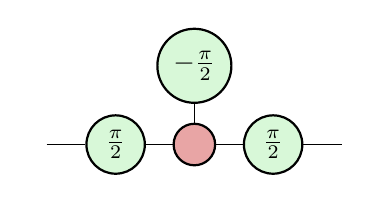
\begin{tikzpicture}
    \node (0) at (0.00, 0.00) {};
    \node [style=gn] (1) at (1, 0) {\(\frac\pi2\)};
    \node [style=gn] (a) at (2,1) {\(-\frac\pi2\)};
    \node [style=rn] (2) at (2, 0) {};
    \node [style=gn] (3) at (3, 0) {\(\frac\pi2\)};
    \node (4) at (4.00, 0.00) {};
    \draw (0) to (1);
    \draw (1) to (2);
    \draw (2) to (3);
    \draw (2) to (a);
    \draw (3) to (4);
    \end{tikzpicture}.
\end{center}
Ker jih bomo pogosto potrebovali, vpeljemo za ta vrata novo oznako
\begin{center}
    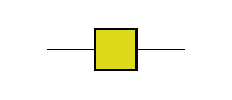
\begin{tikzpicture}
        \node (0) at (0, 0) {};
        \node [style=had] (h) at (1,0) {};
        \node (1) at (2,0) {};
        \draw (0) to (h);
        \draw (h) to (1);
    \end{tikzpicture}.
\end{center}
Kasneje bomo videli, da je, z uporabo teh vrat, diagram
\begin{center}
    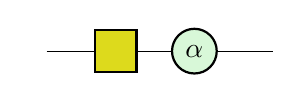
\begin{tikzpicture}
        \node (0) at (0, 0) {};
        \node [style=had] (h) at (1,0) {};
        \node [style=gn] (g) at (2,0) {\(\alpha\)};
        \draw (0) to (h);
        \draw (h) to (g);
        \draw (g) to (3,0);
    \end{tikzpicture}
\end{center}
ekvivalenten diagramu
\begin{center}
    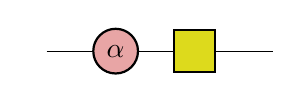
\begin{tikzpicture}
        \node (0) at (0, 0) {};
        \node [style=had] (h) at (2,0) {};
        \node [style=rn] (g) at (1,0) {\(\alpha\)};
        \draw (0) to (g);
        \draw (h) to (g);
        \draw (h) to (3,0);
    \end{tikzpicture}.
\end{center}
Ta lastnost je dejansko ključna za definicijo hadamardovih vrat ter tudi pokaže zakaj so hadamardova vrata pomembna, saj nam omogočajo menjavo baze (iz Z na X ali obratno). Lahko si tudi ogledamo matriko preslikave. Tako hadamardovim vratom ustreza matrika
\begin{align*}
    \frac{1}{\sqrt2}\begin{bmatrix}
        1&1\\
        1&-1
    \end{bmatrix}
\end{align*}

Tako smo definirali osnovne sestavne elemente ZX-diagramov. Brez operacij nad njimi pa so te diagrami le navadni grafi, nepovezani z kvantno mehaniko ali kvantnimi procesi. Dovoljene operacije podamo kot seznam aksiomov, ki pripadajo ZX-računu.
\subsection{Aksiomi}
Za začetek bomo uporabili aksiomatizacijo za splošen ZX-račun podano v \cite[poglavje 2.2]{vilmart}, obstajajo pa tudi nekatere razširitve in drobci, prav tako pa alternativne izbire aksiomov.

Aksiomi ZX diagramov so zelo simetrični. Če neka lastnost velja za diagrame z zelenimi Z pajki, velja tudi, če te pajke spremenimo v rdeče X pajke. Tudi bolj splošno velja: za vsak aksiom obstaja dualni aksiom, kjer so povezave in faze identične, barve pa zamenjamo. Torej lahko zamenjamo tudi barvo pravil, ki vsebujejo mešane pajke (in ne le samo enobarvnih). Dodatno, vsi predstavljeni aksiomi so ekvivalence, torej za njih držijo lastnosti ekvivalenčnih relacij. Posebej je treba poudariti simetričnost: pravila delujejo tudi v obratno smer. Ko aksiom pravi, da lahko sosednje pajke združimo bi prav tako lahko samotarski pajek ločili v več novih (dokler ga lahko z enakim aksiomom združimo nazaj v prvotnega).

Aksiome se ponavadi uporablja kot pravila prepisovanja, podobno kot pri poenostavljanju enačb (le da tukaj poenostavljamo vezja). Tako kot lahko pri enačbah vedno \(1\) zamenjamo z \(\cos(0)\), ne glede na to kje v izrazu se nahaje, lahko tu podgraf zamenjamo z ekvivalentnim podgrafom.

\subsubsection{Topologija} Prvi in ključni aksiom ZX diagramov je, da lahko povezave med pajki poljubno ukrivimo, s tem pa ne spremenimo pomena vezja.
Tako, na primer
\begin{center}
    \begin{tikzpicture}
		\node (0) at (0, 1) {};
		\node (1) at (0, 0) {};
		\node (2) at (2, 0) {}; %left right
		\node (3) at (0, -1) {};
		\node (4) at (-2, 0) {}; %left left
		\node (5) at (10, -1) {};
		\node (6) at (10, 0) {};
		\node (7) at (12, 0) {};
		\node (8) at (10, 1) {};
		\node (9) at (8, 0) {};
		\node (10) at (4, 0) {};
		\node (11) at (6, 0) {};
        \node (leq) at (3,0) {=};
        \node (req) at (7,0) {=};
		\draw [bend right=90, looseness=1.5] (0.center) to (1.center);
		\draw [bend right=15, looseness=1] (2.center) to (0.center);
		\draw [bend left=75, looseness=1.5] (1.center) to (3.center);
		\draw [bend right=-15, looseness=1](3.center) to (4.center);
		\draw [bend left=90, looseness=1.50] (5.center) to (6.center);
		\draw [bend right=-15, looseness=1](7.center) to (5.center);
		\draw [bend right=90, looseness=1.5] (6.center) to (8.center);
		\draw [bend right=15, looseness=1](8.center) to (9.center);
		\draw (10.center) to (11.center);
    \end{tikzpicture}.
\end{center}
Podobno lahko razrešimo vozle
\begin{center}
    \begin{tikzpicture}
        \node (0) at  (0,0) {};
        \node (1) at (2,0) {};
        \node (2) at (2,1) {};
        \node (3) at (0,1) {};
        \node (eq) at (3,0.5) {=};
        \node (0a) at (4,0) {};
        \node (1a) at (6,0) {};
        \node (2a) at (6,1) {};
        \node (3a) at (4,1) {};
        \draw (0.center) -- (1.center) -- (2.center) to (3.center);
        \draw (0a.center) -- (2a.center) -- (1a.center) to (3a.center);
    \end{tikzpicture}.
\end{center}

Zanimivo in pomembno je tudi, da se topološka ekvivalenca prenese na vhode in izhode vrat.
\begin{center}
    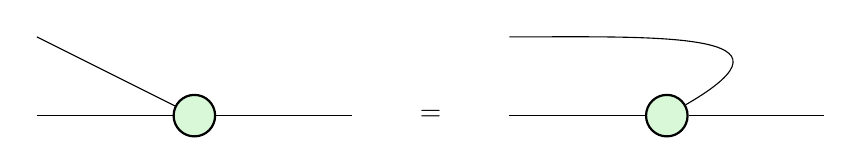
\begin{tikzpicture}
        \node (0) at (0, 1) {};
		\node (1) at (0, 0) {};
		\node[style=gn] (2) at (2, 0) {};
		\node (3) at (4, 0) {};
		\node (4) at (6, 0) {};
		\node[style=gn] (5) at (8, 0) {};
        \node (eq) at (5,0) {\(=\)};
		\node (6) at (10, 0) {};
		\node (7) at (6, 1) {};
        \draw (1.center) to (2);
		\draw (0.center) to (2);
		\draw (2) to (3.center);
		\draw (4.center) to (5);
		\draw (5) to (6.center);
		\draw [in=30, out=0, looseness=2.00] (7.center) to (5);
    \end{tikzpicture}
\end{center}
Torej je težko govoriti o vhodih ali izhodih pajkov, saj lahko vsak vhod spremenimo v izhod (in s tem ne spremenimo vezja) in tudi obratno. Še vedno pa nam to pomaga pri intuiciji in opisu diagramov, tako da povezavam, ki prihajajo iz leve strani, pravimo vhodi, tistim na desni strani pajka pa izhodi. Pogosto pa zaradi lepšega izgleda povezavo pustimo kar navpično. Kot primer si oglejmo vrata C--NOT. 
\begin{center}
    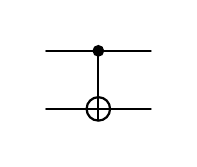
\begin{tikzpicture}
        \node (quantum) at (0,0.5) {
          \begin{quantikz}
            \qw & \ctrl{1} & \qw \\
            \qw & \targ{}  & \qw
          \end{quantikz}
        };
        \end{tikzpicture}
\end{center}
V ZX lahko ta vrata napišemo kot katerikoli izmed slednjih diagramov.
\begin{center}
    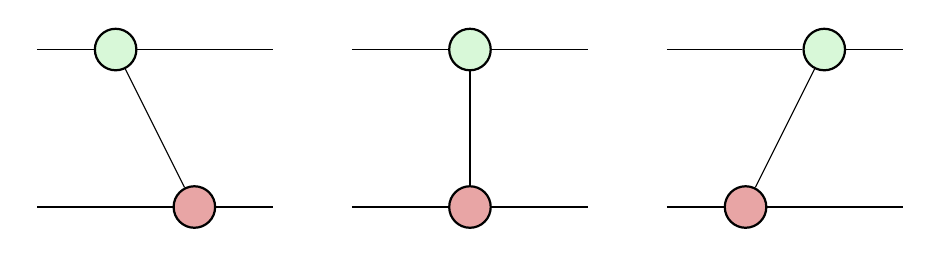
\begin{tikzpicture}
            \node [style=none] (2) at (-2, 1) {};
            \node [style=none] (3) at (-2, -1) {};
            \node [style=none] (4) at (1, 1) {};
            \node [style=none] (5) at (1, -1) {};
            \node [style=none] (6) at (2, 1) {};
            \node [style=none] (7) at (2, -1) {};
            \node [style=none] (8) at (-3, 1) {};
            \node [style=none] (9) at (-3, -1) {};
            \node [style=none] (10) at (-6, -1) {};
            \node [style=none] (11) at (-6, 1) {};
            \node [style=none] (12) at (5, 1) {};
            \node [style=none] (13) at (5, -1) {};
            \node [style=gn] (14) at (-5, 1) {};
            \node [style=gn] (15) at (4, 1) {};
            \node [style=gn] (16) at (-0.5, 1) {};
            \node [style=rn] (17) at (-4, -1) {};
            \node [style=rn] (18) at (-0.5, -1) {};
            \node [style=rn] (19) at (3, -1) {};
            \draw (11.center) to (14);
            \draw (14) to (8.center);
            \draw (14) to (17);
            \draw (17) to (9.center);
            \draw (17) to (10.center);
            \draw (2.center) to (16);
            \draw (16) to (4.center);
            \draw (16) to (18);
            \draw (3.center) to (18);
            \draw (18) to (5.center);
            \draw (6.center) to (15);
            \draw (15) to (12.center);
            \draw (15) to (19);
            \draw (7.center) to (19);
            \draw (19) to (13.center);
    \end{tikzpicture}    
\end{center}
Opazimo, da smo lahko pajek premaknili tudi naprej ali nazaj. Dovoljeno je poljubno premikanje pajkov po ravnini, dokler ne spremenimo kako so povezani.

Ta pravila skupaj nam upravičijo uporabo matematičnih grafov, kot poznanih iz teorije grafov. Tam lahko prav tako vozlišča premikamo po ravnini, povezave lahko ukrivljamo, prav tako pa ni pomembno v katero stran vozlišča vodi povezava, dokler je le pripeta. Pogosto je uporabljen slogan ``\emph{only connectivity matters}'' -- glede oblike so pomembne samo povezave.

Treba pa je poudariti, da v ostalih aksiomih prostega konca vhodnih in izhodnih povezav ne smemo premikati. Razlog je ravno v tem, da aksiome uporabljamo kot pravila prepisovanja; prosti konec povezave je le ena polovica povezave, ki je vidna v našem podgrafu (druga polovica pa se nahaja v grafu, ki ga poenostavljamo). Če bi premikali tudi prosti konec bi lahko močno spremenili pomen. Poglejmo si na primeru, kjer smo ohranili vse povezave, premaknili smo le proste konce.
\begin{center}
    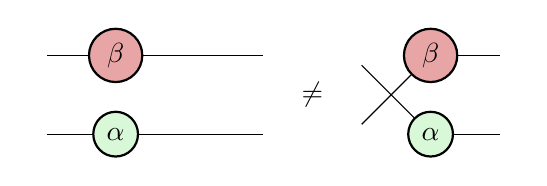
\begin{tikzpicture}
        \node (0) at (0,0) {};
        \node[style=gn] (1) at (1,0) {\(\alpha\)};
        \node[style=rn] (2) at (1,1) {\(\beta\)};
        \node (3) at (0,1) {};
        \node (0a) at (4,0) {};
        \node[style=gn] (1a) at (5,0) {\(\alpha\)};
        \node[style=rn] (2a) at (5,1) {\(\beta\)};
        \node (3a) at (4,1) {};
        \node (neq) at (3.5,0.5) {\(\neq\)};
        \node (end1) at (3,0) {};
        \node (end2) at (3,1) {};
        \node (end3) at (6,0) {};
        \node (end4) at (6,1) {};        
        \draw (0) to (1);
        \draw (2) to (3);
        \draw (0a) to (2a);
        \draw (1a) to (3a);
        \draw (1) to (end1);
        \draw (2) to (end2);
        \draw (1a) to (end3);
        \draw (2a) to (end4);
    \end{tikzpicture}
\end{center}
Če bi poskusili to pravilo uporabiti v diagramu 
\begin{center}
    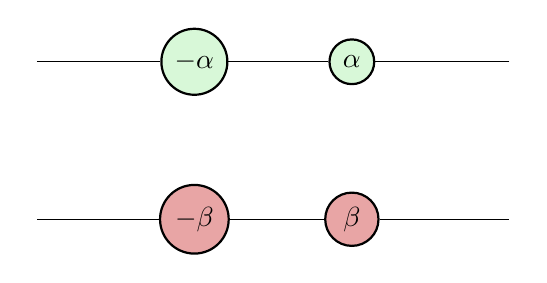
\begin{tikzpicture}
            \node [style=gn] (0) at (-1, 1) {\(-\alpha\)};
            \node [style=gn] (1) at (1, 1) {\(\alpha\)};
            \node [style=rn] (2) at (-1, -1) {\(-\beta\)};
            \node [style=rn] (3) at (1, -1) {\(\beta\)};
            \node [style=none] (4) at (-3, 1) {};
            \node [style=none] (5) at (-3, -1) {};
            \node [style=none] (6) at (3, 1) {};
            \node [style=none] (7) at (3, -1) {};
            \draw (4.center) to (0);
            \draw (0) to (1);
            \draw (6.center) to (1);
            \draw (3) to (7.center);
            \draw (3) to (2);
            \draw (2) to (5.center);
    \end{tikzpicture},
\end{center}
bi dobili
\begin{center}
    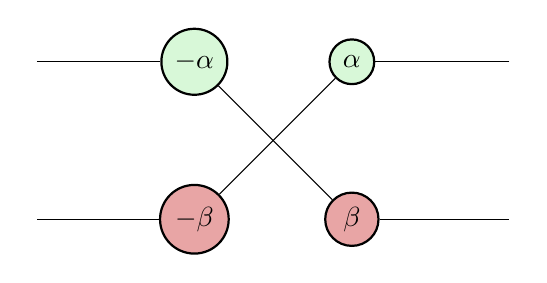
\begin{tikzpicture}
            \node [style=gn] (0) at (-1, 1) {\(-\alpha\)};
            \node [style=gn] (1) at (1, 1) {\(\alpha\)};
            \node [style=rn] (2) at (-1, -1) {\(-\beta\)};
            \node [style=rn] (3) at (1, -1) {\(\beta\)};
            \node [style=none] (4) at (-3, 1) {};
            \node [style=none] (5) at (-3, -1) {};
            \node [style=none] (6) at (3, 1) {};
            \node [style=none] (7) at (3, -1) {};
            \draw (4.center) to (0);
            \draw (6.center) to (1);
            \draw (3) to (7.center);
            \draw (2) to (5.center);
            \draw (0) to (3);
            \draw (1) to (2);
    \end{tikzpicture}
\end{center}
oziroma 
\begin{center}
    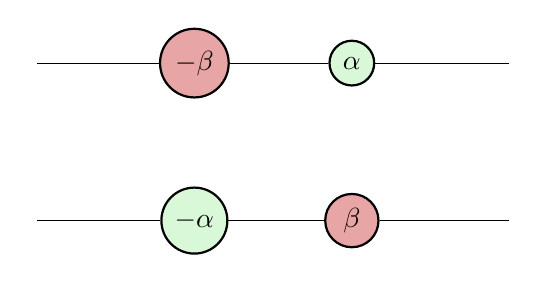
\begin{tikzpicture}
            \node [style=gn] (0) at (-1, -1) {\(-\alpha\)};
            \node [style=gn] (1) at (1, 1) {\(\alpha\)};
            \node [style=rn] (2) at (-1, 1) {\(-\beta\)};
            \node [style=rn] (3) at (1, -1) {\(\beta\)};
            \node [style=none] (4) at (-3, -1) {};
            \node [style=none] (5) at (-3, 1) {};
            \node [style=none] (6) at (3, 1) {};
            \node [style=none] (7) at (3, -1) {};
            \draw (4.center) to (0);
            \draw (6.center) to (1);
            \draw (3) to (7.center);
            \draw (2) to (5.center);
            \draw (0) to (3);
            \draw (1) to (2);
    \end{tikzpicture}.
\end{center}
Kar pa za večino faz ne bo ekvivalentno! Izvorni diagram namreč je ekvivalenten identiteti (za kar potrebujemo še nekaj dodatnih aksiomov), izpeljani pa za recimo \(\alpha = \beta = \frac\pi2\) ni.

Torej si predstavljamo, da so prosti konci togo vpeti v ravnino (ali pa da vsaj ohranijo isto povezavo v nadgrafu, ko uporabimo pravilo).
% ----------------------------- aksiomi --------------------------------------------------------------------------------
\subsubsection{Identiteta} \label{identiteta}
Če imamo pajek z natanko enim vhodom in izhodom, je to vezje ekvivalentno identiti
\begin{center}
    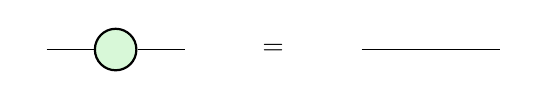
\begin{tikzpicture}
        \node (1) at (0,0) {};
        \node[style=gn] (gn) at (1,0) {};
        \node (2) at (2,0) {};
        \node (eq) at (3,0) {\(=\)};
        \node (4) at (4,0) {};
        \node (5) at (6,0) {};
        \draw (1) to (gn) to (2); 
        \draw (4) to (5);
    \end{tikzpicture}
\end{center}

\subsubsection{Združitev pajkov} \label{zdruzitev}
Sosednje pajke iste barve lahko združimo dokler ohranimo isto število skupnih vhodov in izhodov. Pri tem se faze seštejejo.
\begin{center}
    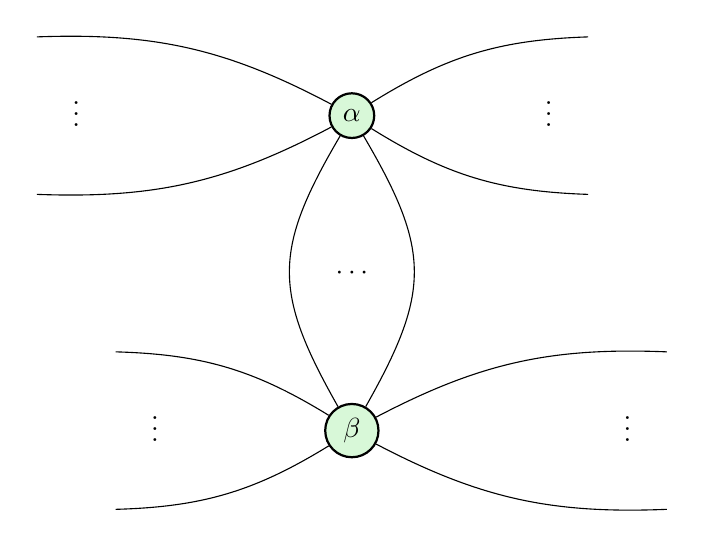
\begin{tikzpicture}
        \node [style=gn] (0) at (0, 2) {\(\alpha\)};
        \node [style=gn] (1) at (0, -2) {\(\beta\)};
        \node [style=none] (2) at (4, -1) {};
        \node [style=none] (3) at (4, -3) {};
        \node [style=none] (4) at (-4, 3) {};
        \node [style=none] (5) at (-4, 1) {};
        \node [style=none] (6) at (3, 3) {};
        \node [style=none] (7) at (3, 1) {};
        \node [style=none] (8) at (-3, -1) {};
        \node [style=none] (9) at (-3, -3) {};
        \node [style=none] (10) at (2.5, 2) {\(\rvdots\)};
        \node [style=none] (12) at (-2.5, -2) {\(\rvdots\)};
        \node [style=none] (13) at (3.5, -2) {\(\rvdots\)};
        \node [style=none] (14) at (0, 0) {\(\cdots\)};
        \node [style=none] (15) at (-3.5, 2) {\(\rvdots\)};
        \draw [bend left=15] (4.center) to (0);
        \draw [bend right=15] (5.center) to (0);
        \draw [bend right=15] (2.center) to (1);
        \draw [bend left=15] (3.center) to (1);
        \draw [bend right, looseness=1.25] (0) to (1);
        \draw [bend left, looseness=1.25] (0) to (1);
        \draw [bend left=15] (0) to (6.center);
        \draw [bend right=15] (0) to (7.center);
        \draw [bend left=15] (8.center) to (1);
        \draw [bend right=15] (9.center) to (1);
    \end{tikzpicture}
\end{center}
lahko prepišemo v
\begin{center}
    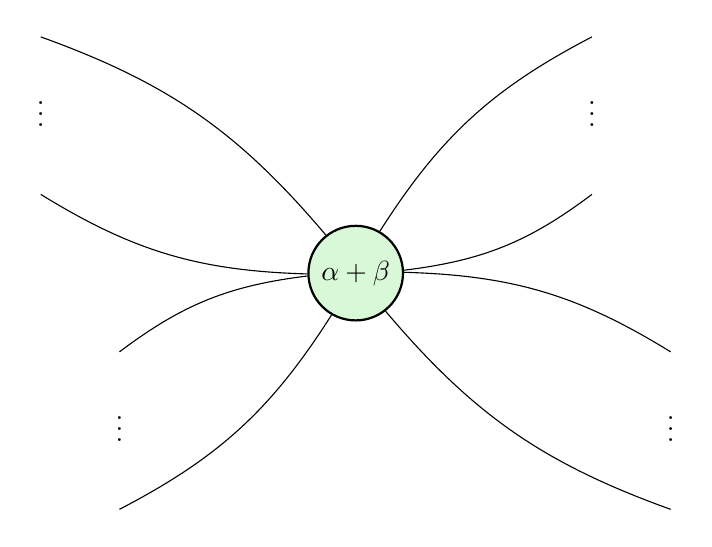
\begin{tikzpicture}
            \node [style=gn] (0) at (0, 0) {\(\alpha+\beta\)};
            \node [style=none] (1) at (-4, 3) {};
            \node [style=none] (2) at (-4, 1) {};
            \node [style=none] (3) at (-3, -1) {};
            \node [style=none] (4) at (-3, -3) {};
            \node [style=none] (5) at (4, -1) {};
            \node [style=none] (6) at (4, -3) {};
            \node [style=none] (7) at (3, 3) {};
            \node [style=none] (8) at (3, 1) {};
            \node [style=none] (9) at (-4, 2) {\(\rvdots\)};
            \node [style=none] (10) at (-3, -2) {\(\rvdots\)};
            \node [style=none] (11) at (3, 2) {\(\rvdots\)};
            \node [style=none] (12) at (4, -2) {\(\rvdots\)};
            \draw [bend left=15] (1.center) to (0);
            \draw [bend right=15] (2.center) to (0);
            \draw [bend left=15] (3.center) to (0);
            \draw [bend right=15] (4.center) to (0);
            \draw [bend right=15] (7.center) to (0);
            \draw [bend left=15] (8.center) to (0);
            \draw [bend right=15] (5.center) to (0);
            \draw [bend left=15] (6.center) to (0);
    \end{tikzpicture}.
\end{center}
Med pajkoma more biti vsaj ena povezava, pravih vhodov ali izhodov pa je lahko tudi nič.

Aksioma za združitev pajkov in identiteto ustrezata aksiomatizaciji ortonormirane baze \cite[poglavje 5]{coecke_pavlovic_vicary_2013}.

\subsubsection{Izničenje pajkov} \label{iznicenje}
Povezani pajki določenih baz so ekvivalentni praznemu diagramu. Diagrame oblike
\begin{center}
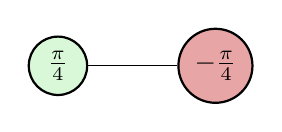
\begin{tikzpicture}
		\node [style=rn] (0) at (2, 0) {\(-\frac\pi4\)};
		\node [style=gn] (1) at (0,0) {\(\frac\pi4\)};
		\draw (0) to (1);
\end{tikzpicture}
\end{center}
lahko preprosto izbrišemo. Prazen diagram ustreza skalarju \(1\), torej je ta diagram ekvivalenten skalarju. To je edini aksiom, ki nam lahko ustvari prazen diagram.

Kot zanimivost, podvojeno verzija tega pravila lahko izpeljemo tudi brez zgornjega pravila \cite[poglavje 3.1]{jeandel_et_al}! Tako je tudi
\begin{center}
    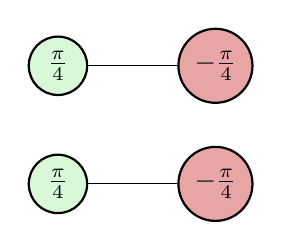
\begin{tikzpicture}
            \node [style=rn] (0) at (2, 0) {\(-\frac\pi4\)};
            \node [style=gn] (1) at (0, 0) {\(\frac\pi4\)};
            \node [style=rn] (00) at (2, 1.5) {\(-\frac\pi4\)};
            \node [style=gn] (11) at (0, 1.5) {\(\frac\pi4\)};
            \draw (0) to (1);
            \draw (00) to (11);
    \end{tikzpicture}
\end{center}
ekvivalenten skalarju \(1\)

\subsubsection{Bialgebra} \label{bialgebra}
Prvo izmed pravil, ki izraža močno komplementarnost baz je pravilo bialgebre.
\begin{center}
    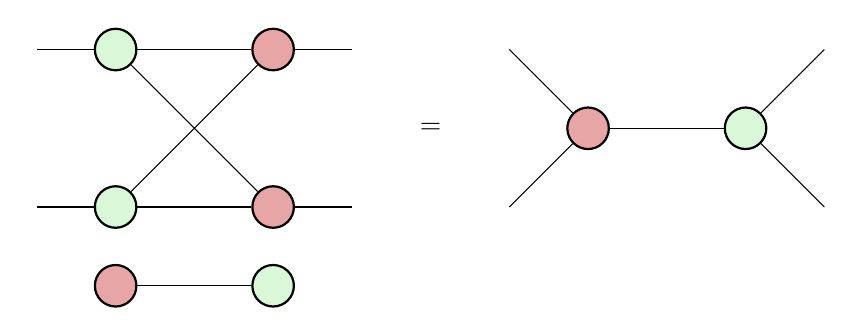
\begin{tikzpicture}
            \node [style=gn] (0) at (-3, 0) {};
            \node [style=gn] (1) at (-3, 2) {};
            \node [style=gn] (2) at (-1, -1) {};
            \node [style=rn] (3) at (-3, -1) {};
            \node [style=rn] (4) at (-1, 0) {};
            \node [style=rn] (5) at (-1, 2) {};
            \node [style=none] (6) at (-4, 0) {};
            \node [style=none] (7) at (-4, 2) {};
            \node [style=none] (8) at (0, 0) {};
            \node [style=none] (9) at (0, 2) {};
            \node [style=none] (10) at (1, 1) {\(=\)};
            \node [style=rn] (11) at (3, 1) {};
            \node [style=gn] (12) at (5, 1) {};
            \node [style=none] (13) at (2, 0) {};
            \node [style=none] (14) at (2, 2) {};
            \node [style=none] (15) at (6, 0) {};
            \node [style=none] (16) at (6, 2) {};
            \draw (6.center) to (0);
            \draw (7.center) to (1);
            \draw (0) to (4);
            \draw (4) to (8.center);
            \draw (1) to (5);
            \draw (5) to (9.center);
            \draw (3) to (2);
            \draw (0) to (5);
            \draw (1) to (4);
            \draw (11) to (12);
            \draw (12) to (15.center);
            \draw (12) to (16.center);
            \draw (11) to (14.center);
            \draw (11) to (13.center);
    \end{tikzpicture}    
\end{center}

\subsubsection{Pravilo kopiranja} \label{kopiranje}
Drugo pravilo močne komplementarnosti baz nam omogoča, da vhod ``kopiramo''. Izvorna informacija prihaja iz enega rdečega pajka naprej, s tem pravilom pa je to ekvivalentno dvem pajkom
\begin{center}
    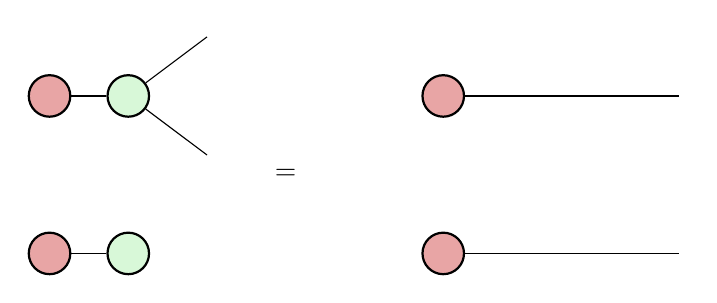
\begin{tikzpicture}
            \node [style=rn] (0) at (-3, -1) {};
            \node [style=rn] (1) at (-3, 1) {};
            \node [style=gn] (2) at (-2, -1) {};
            \node [style=gn] (3) at (-2, 1) {};
            \node [style=none] (4) at (-1, 0.25) {};
            \node [style=none] (5) at (-1, 1.75) {};
            \node [style=none] (7) at (0, 0) {\(=\)};
            \node [style=rn] (8) at (2, -1) {};
            \node [style=rn] (9) at (2, 1) {};
            \node [style=none] (10) at (5, -1) {};
            \node [style=none] (11) at (5, 1) {};
            \draw (0) to (2);
            \draw (1) to (3);
            \draw (3) to (4.center);
            \draw (3) to (5.center);
            \draw (8) to (10.center);
            \draw (9) to (11.center);
    \end{tikzpicture}      
\end{center}

\subsubsection{Hadamardova dekompozicija} \label{had-dekomp}
Lahko naredimo dekompozicijo hadamardovih vrat z uporabo \(\frac\pi2\) rotacij.
\begin{center}
    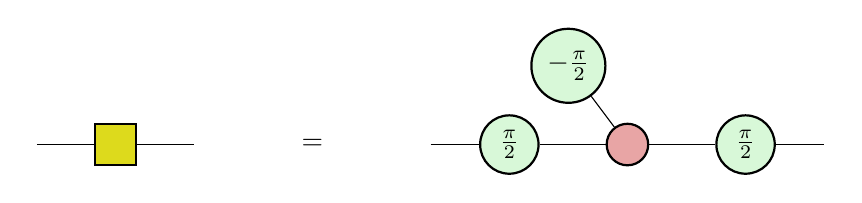
\begin{tikzpicture}
        \node [style=none] (0) at (-5, 0) {};
		\node [style=none] (1) at (-3, 0) {};
		\node [style=had] (2) at (-4, 0) {};
		\node [style=none] (4) at (-1.5, 0) {\(=\)};
		\node [style=none] (5) at (0, 0) {};
		\node [style=none] (6) at (5, 0) {};
		\node [style=rn] (7) at (2.5, 0) {};
		\node [style=gn] (8) at (1, 0) {\(\frac\pi2\)};
		\node [style=gn] (9) at (4, 0) {\(\frac\pi2\)};
		\node [style=gn] (10) at (1.75, 1) {\(-\frac\pi2\)};
		\draw (0.center) to (2);
		\draw (2) to (1.center);
		\draw (5.center) to (8);
		\draw (8) to (7);
		\draw (7) to (9);
		\draw (9) to (6.center);
		\draw (7) to (10);
    \end{tikzpicture}    
\end{center}

\subsubsection{Hadamardova menjava barv} \label{had-menjava}
Hadamardova vrata lahko uporabimo za menjavo barve pajka tako, da na vse njegove vhode in izhode dodamo hadamardova vrata ter zamenjamo barvo.
\begin{center}
    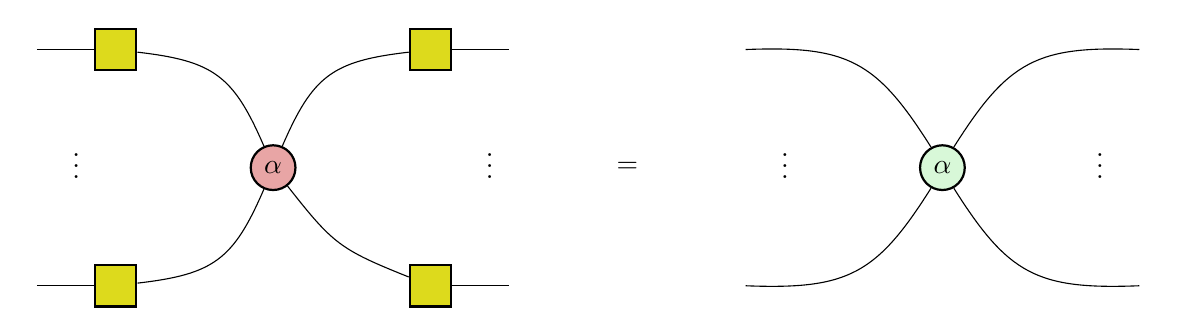
\begin{tikzpicture}
            \node [style=none] (0) at (-8, -1.5) {};
            \node [style=none] (1) at (-8, 1.5) {};
            \node [style=none] (2) at (-2, 1.5) {};
            \node [style=none] (3) at (-2, -1.5) {};
            \node [style=rn] (5) at (-5, 0) {\(\alpha\)};
            \node [style=had] (6) at (-7, -1.5) {};
            \node [style=had] (7) at (-7, 1.5) {};
            \node [style=had] (8) at (-3, 1.5) {};
            \node [style=had] (9) at (-3, -1.5) {};
            \node [style=none] (11) at (-0.5, 0) {\(=\)};
            \node [style=gn] (13) at (3.5, 0) {\(\alpha\)};
            \node [style=none] (14) at (6, 1.5) {};
            \node [style=none] (15) at (6, -1.5) {};
            \node [style=none] (16) at (1, -1.5) {};
            \node [style=none] (17) at (1, 1.5) {};
            \node [style=none] (18) at (-2.25, 0) {\(\rvdots\)};
            \node [style=none] (19) at (5.5, 0) {\(\rvdots\)};
            \node [style=none] (20) at (-7.5, 0) {\(\rvdots\)};
            \node [style=none] (21) at (1.5, 0) {\(\rvdots\)};
            \draw (0.center) to (6);
            \draw (1.center) to (7);
            \draw (8) to (2.center);
            \draw (9) to (3.center);
            \draw [bend right, looseness=1.25] (13) to (17.center);
            \draw [bend left, looseness=1.25] (13) to (16.center);
            \draw [bend right, looseness=1.25] (13) to (15.center);
            \draw [bend left, looseness=1.25] (13) to (14.center);
            \draw [bend right, looseness=1.25] (6) to (5);
            \draw [bend left, looseness=1.25] (7) to (5);
            \draw [bend left=15, looseness=1.25] (9) to (5);
            \draw [bend right, looseness=1.25] (8) to (5);
    \end{tikzpicture}    
\end{center}

Ta aksiom karakterizira Hadamardova vrata glede na to, kako spreminja pajke oziroma kako vpliva na preostanek diagrama, med tem ko prejšnji aksiom karakterizira vrata glede na to kaj vrata so na elementaren način, neodvisno od preostanka diagrama. Prejšnji opisuje kaj Hadamardova so, ta pa kaj naredijo.

\subsubsection{Eulerjevi koti} \label{euler}
Zadnji aksiom je tudi najtežji in tudi najbolj nestandarden, vendar potreben za določene zaželjene lastnosti lastnosti, še posebaj polnost (če imamo par diagramov, ki predstavljata isti kvantni proces sta tudi ekvivalentna - lahko enega pretvorimo v drugega z uporabo aksiomov). 
\begin{center}
    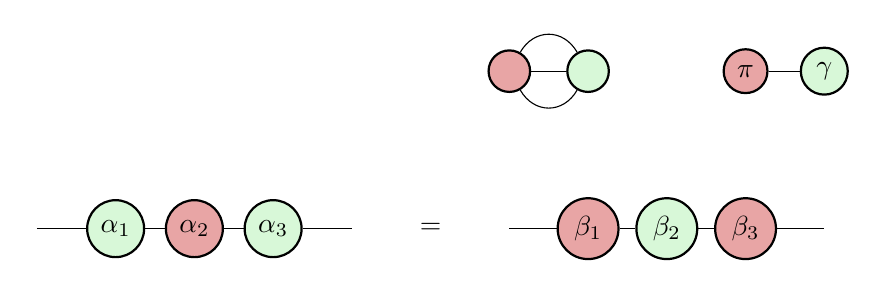
\begin{tikzpicture}
            \node [style=none] (0) at (-4, 0) {};
            \node [style=gn] (1) at (-3, 0) {\(\alpha_1\)};
            \node [style=gn] (2) at (-1, 0) {\(\alpha_3\)};
            \node [style=rn] (3) at (-2, 0) {\(\alpha_2\)};
            \node [style=none] (4) at (0, 0) {};
            \node [style=none] (5) at (1, 0) {\(=\)};
            \node [style=none] (6) at (2, 0) {};
            \node [style=none] (7) at (6, 0) {};
            \node [style=gn] (8) at (4, 0) {\(\beta_2\)};
            \node [style=rn] (9) at (5, 0) {\(\beta_3\)};
            \node [style=rn] (10) at (3, 0) {\(\beta_1\)};
            \node [style=rn] (11) at (2, 2) {};
            \node [style=gn] (12) at (3, 2) {};
            \node [style=rn] (13) at (5, 2) {\(\pi\)};
            \node [style=gn] (14) at (6, 2) {\(\gamma\)};
            \draw (0.center) to (1);
            \draw (1) to (3);
            \draw (3) to (2);
            \draw (2) to (4.center);
            \draw [bend left=60, looseness=1.25] (11) to (12);
            \draw [bend right=60, looseness=1.25] (11) to (12);
            \draw (11) to (12);
            \draw (13) to (14);
            \draw (6.center) to (10);
            \draw (10) to (8);
            \draw (8) to (9);
            \draw (9) to (7.center);
    \end{tikzpicture}    
\end{center}
Na levi strani enakosti imamo dane poljubne \(\alpha_1,\alpha_2,\alpha_3\), na desni strani pa moremo vrednosti izračunati. Definiramo si nekaj pomožnih vrednosti.
\begin{align*}
    x^+ \defeq \frac{\alpha_1 + \alpha_3}{2}\\
    x^- \defeq x^+-\alpha_3\\
    z \defeq \cos\left(\frac{\alpha_2}{2}\right)\cos\left(x^+\right) + i\sin\left(\frac{\alpha_2}{2}\right)\cos\left(x^-\right)\\
    z' \defeq \cos\left(\frac{\alpha_2}{2}\right)\sin\left(x^+\right) - i\sin\left(\frac{\alpha_2}{2}\right)\sin\left(x^-\right)
\end{align*}
Z njihovo pomočjo lahko izračunamo ostale parametre
\begin{align*}
    \beta_1 = \arg z + \arg z'\\
    \beta_2 = 2\arg\left(i+\left\lvert\frac{z}{z'}\right\rvert\right)\\
    \beta_3 = \arg z - \arg z'\\
    \gamma = x^+-\arg z + \frac{\alpha_2-\beta_2}{2}
\end{align*}
Po dogovoru vzamemo tako funkcijo \(\arg\), da \(\arg(0)=0\). Če je \(z'=0\) pa definiramo \(\beta_2 = 0\).

Motivacija za ta aksiom prihaja iz Eulerjevih kotov poznanih iz klasične analize. Te nam omogočijo dekompozicijo poljubne rotacije kot kompozicijo rotacij okoli standardnih koordinatnih osi. Enako lahko povemo v jeziku linearne algebre: poljubno rotacijsko matriko \(R\) lahko napišemo kot \(R=X(\alpha)Y(\beta)Z(\gamma)\). Ta izrek ima v kvantni mehaniki pomembno posledico, namreč omogoča nam da lahko zapišemo poljuben unitarni operator enega kubita kot kompozicijo rotacij okoli \(Z,X,Z\) ali okoli \(X,Z,X\), ta aksiom pa nam definira, da sta dve dekompoziciji istega unitarnega operatorja ekvivalentna.

Ta aksiom je poseben tudi v tem, da so ostali aksiomi linearni, ta pa je nelinearen. To vidimo že iz tega, da faze dobljenih pajkov niso linearne kombinacije ostalih faz, pač pa tukaj uporabimo tudi nelinearne kotne funkcije ter argument. Vendar pa je prav zato potreben za polnost jezika, saj je namreč znano da različica ZX-računa brez nelinearnega aksioma ne more biti polna \cite[izrek 6.1]{jeandeldiagrammatic}.

\subsection{Primeri}
Za lažje razumevanje podanih aksiomov si poglejmo nekaj primerov in izrekov v ZX-računu, ki jih lahko dokažemo.
\subsubsection{Hadamard je sam sebi inverz}
Inverz diagrama \(D:n\to n\) je diagram \(D^{-1}:n\to n\), da \(D\circ D^{-1} = D^{-1}\circ D = \bigotimes{i=1}^n\id\). Tukaj je identiteta \(\id\) samo povezava od vhoda do izhoda brez pajka; diagramu ustreza identična matrika \(\interpret{\bigotimes_{i=1}^n\id} = I = (\delta_{ij})_{i,j=1,\ldots 2^n}\). Že kot aksiom imamo podano to, da je pajek brez faze ekvivalenten identiteti, kar posledično pomeni, da je sam svoj inverz. Podobno velja tudi za Hadamardova vrata \(H\). Ta niso ekvivalentna identiteti, velja pa, da so svoj inverz \(H\circ H = \id\).
\begin{center}
    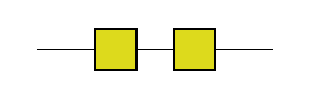
\begin{tikzpicture}
            \node [style=none] (0) at (-1, 0) {};
            \node [style=none] (1) at (2, 0) {};
            \node [style=had] (2) at (0, 0) {};
            \node [style=had] (3) at (1, 0) {};
            \draw (0.center) to (2);
            \draw (2) to (3);
            \draw (3) to (1.center);
    \end{tikzpicture}    
\end{center}
Uporabimo aksiom o identiteti \ref{identiteta}, ki pove, da je (prazna) povezava ekvivalentna povezavi z pajkom, ki ima fazo 0. To lahko uporabimo na povezavi med Hadamardovima vratoma, da vstavimo nov pajek in dobimo ekvivalentno vezje.
\begin{center}
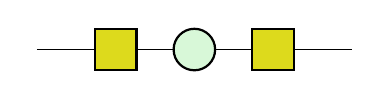
\begin{tikzpicture}
		\node [style=none] (0) at (-1, 0) {};
		\node [style=none] (1) at (3, 0) {};
		\node [style=had] (2) at (0, 0) {};
		\node [style=had] (3) at (2, 0) {};
		\node [style=gn] (4) at (1, 0) {};
		\draw (0.center) to (2);
		\draw (3) to (1.center);
		\draw (2) to (4);
		\draw (4) to (3);
\end{tikzpicture}
\end{center}
Temu sledi uporaba Hadamardove menjave barv \ref{had-menjava}.
\begin{center}
    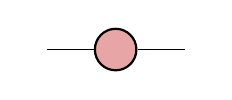
\begin{tikzpicture}
        \node [style=none] (0) at (0,0) {};
        \node [style=rn] (1) at (1,0) {};
        \node [style=none] (2) at (2,0) {};
        \draw (0) to (1);
        \draw (1) to (2);
    \end{tikzpicture}
\end{center}
Nazadnje spet uporabimo aksiom o identiteti \ref{identiteta}, kar nam poda identično preslikavo.
\begin{center}
    \begin{tikzpicture}
        \node [style=none] (0) at (0,0) {};
        \node [style=none] (2) at (2,0) {};
        \draw (0) to (2);
    \end{tikzpicture}
\end{center}
Tako smo dokazali, da so Hadamardova vrata sama svoj inverz. Ta izrek lahko uporabimo v naslednjem primeru.
\subsubsection{Hadamard menja barve}
V uvodu v ZX-račun smo v omenili, da velja
\begin{center}
    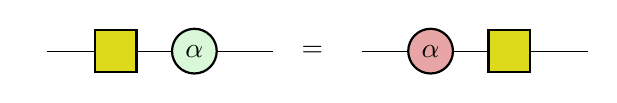
\begin{tikzpicture}
        \node (0) at (0, 0) {};
        \node [style=had] (h) at (1,0) {};
        \node [style=gn] (g) at (2,0) {\(\alpha\)};
        \node (0a) at (4, 0) {};
        \node (=) at (3.5,0) {\(=\)}; 
        \node [style=had] (ha) at (6,0) {};
        \node [style=rn] (ga) at (5,0) {\(\alpha\)};
        \draw (0) to (h);
        \draw (h) to (g);
        \draw (g) to (3,0);
        \draw (0a) to (ga);
        \draw (ha) to (ga);
        \draw (ha) to (7,0);
    \end{tikzpicture}.
\end{center}
Začnemo z levo stranjo enakosti in na njej uporabimo prejšnji izrek.
\begin{center}
    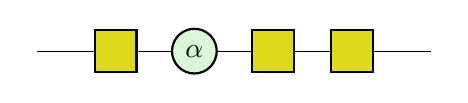
\begin{tikzpicture}
            \node [style=none] (0) at (-1, 0) {};
            \node [style=had] (2) at (0, 0) {};
            \node [style=gn] (4) at (1, 0) {\(\alpha\)};
            \node [style=had] (5) at (2, 0) {};
            \node [style=had] (6) at (3, 0) {};
            \node [style=none] (7) at (4, 0) {};
            \draw (0.center) to (2);
            \draw (2) to (4);
            \draw (4) to (5);
            \draw (5) to (6);
            \draw (6) to (7.center);
    \end{tikzpicture}    
\end{center}
Tako smo dobili diagram, na katerem lahko uporabimo Hadamardovo menjavo barv \ref{had-menjava}.
\begin{center}
    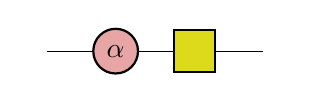
\begin{tikzpicture}
        \node [style=none] (0) at (0,0) {};
        \node [style=rn] (1) at (1,0) {\(\alpha\)};
        \node [style=had] (2) at (2,0) {};
        \node [style=none] (3) at (3,0) {};
        \draw (0) to (1);
        \draw (1) to (2);
        \draw (2) to (3);
    \end{tikzpicture}
\end{center}
\subsubsection{Hopfov zakon} \label{hopf}
Hopfov zakon je teoretično zanimiv, saj pove, da je komplementarnost posledica močne komplementarnosti.
\begin{center}
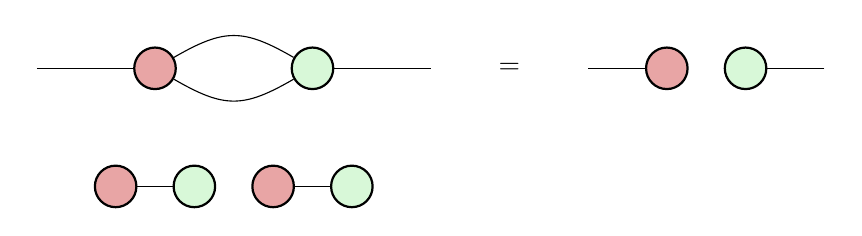
\begin{tikzpicture}
		\node [style=rn] (0) at (-0.5, 0) {};
		\node [style=rn] (1) at (-1, -1.5) {};
		\node [style=rn] (2) at (1, -1.5) {};
		\node [style=gn] (3) at (1.5, 0) {};
		\node [style=gn] (4) at (0, -1.5) {};
		\node [style=gn] (5) at (2, -1.5) {};
		\node [style=none] (6) at (-2, 0) {};
		\node [style=none] (7) at (3, 0) {};
		\node [style=none] (8) at (4, 0) {\(=\)};
		\node [style=none] (9) at (5, 0) {};
		\node [style=none] (10) at (8, 0) {};
		\node [style=rn] (11) at (6, 0) {};
		\node [style=gn] (12) at (7, 0) {};
		\draw [bend left, looseness=1.25] (0) to (3);
		\draw (1) to (4);
		\draw (2) to (5);
		\draw [bend right, looseness=1.25] (0) to (3);
		\draw (6.center) to (0);
		\draw (3) to (7.center);
		\draw (9.center) to (11);
		\draw (10.center) to (12);
\end{tikzpicture}
\end{center}
Za induicijo sledimo toku podatkov. Na levi strani enačbe imamo povezavo od X pajka do Z pajka, na desni strani enačbe pa vhod pride do X pajka, se pozabi, Z pajek pa se na novo (neodvisno) izmisli nove podatke, ter jih pošlje naprej. To je posledica tega, da sta X in Z pajka v različni bazi - če najprej izmerimo spin v X smeri in potem v Z smeri smo izgubili prvotno informacijo \cite[definicija 8.27]{coecke_kissinger_2017}. V praksi pa nam dovoli, da razbijemo povezan diagram na nepovezane dele in ga tako poenostavimo.

Pravilo je posledica aksioma bialgebre \cite[poglavje 3.2.3]{Backens}. Začnemo na levi strani enakosti ter dvakrat uporabimo aksiom o identiteti \ref{identiteta}.
\begin{center}
    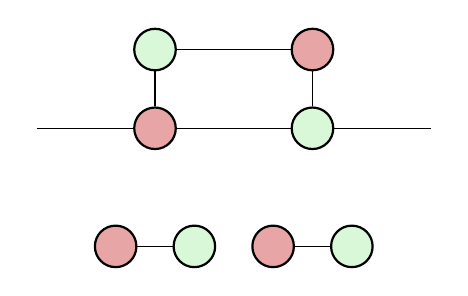
\begin{tikzpicture}
            \node [style=rn] (0) at (-0.5, 0) {};
            \node [style=rn] (1) at (-1, -1.5) {};
            \node [style=rn] (2) at (1, -1.5) {};
            \node [style=gn] (3) at (1.5, 0) {};
            \node [style=gn] (4) at (0, -1.5) {};
            \node [style=gn] (5) at (2, -1.5) {};
            \node [style=none] (6) at (-2, 0) {};
            \node [style=none] (7) at (3, 0) {};
            \node [style=rn] (8) at (1.5, 1) {};
            \node [style=gn] (9) at (-0.5, 1) {};
            \draw (1) to (4);
            \draw (2) to (5);
            \draw (0) to (3);
            \draw (6.center) to (0);
            \draw (3) to (7.center);
            \draw (9) to (0);
            \draw (9) to (8);
            \draw (8) to (3);
    \end{tikzpicture}    
\end{center}
Sedaj le topološko preuredimo graf, da ima bolj znano obliko
\begin{center}
    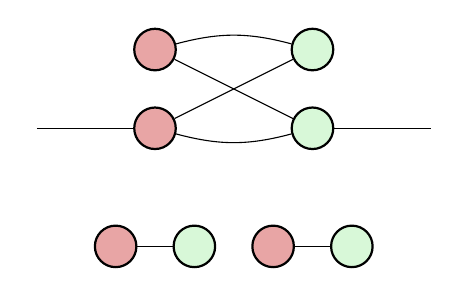
\begin{tikzpicture}
            \node [style=rn] (0) at (-0.5, 0) {};
            \node [style=rn] (1) at (-1, -1.5) {};
            \node [style=rn] (2) at (1, -1.5) {};
            \node [style=gn] (3) at (1.5, 0) {};
            \node [style=gn] (4) at (0, -1.5) {};
            \node [style=gn] (5) at (2, -1.5) {};
            \node [style=none] (6) at (-2, 0) {};
            \node [style=none] (7) at (3, 0) {};
            \node [style=rn] (8) at (-0.5, 1) {};
            \node [style=gn] (9) at (1.5, 1) {};
            \draw (1) to (4);
            \draw (2) to (5);
            \draw [bend right=15] (0) to (3);
            \draw (6.center) to (0);
            \draw (3) to (7.center);
            \draw (9) to (0);
            \draw [bend left=345] (9) to (8);
            \draw (8) to (3);
    \end{tikzpicture}    
\end{center}
Uporabimo aksiom o združitvi \ref{zdruzitev} v obratno smer - že združena pajka (oba z fazo \(0\)) ločimo narazen. Novi pajek ne bo imel vhodov ali izhodov, le povezavo do drugega pajka, katerega je bil del.
\begin{center}
    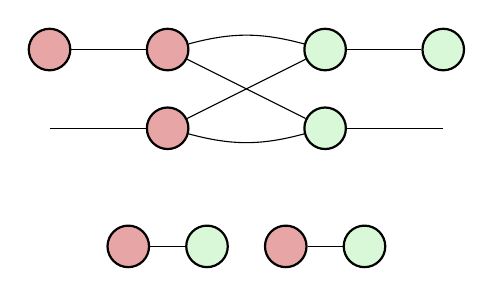
\begin{tikzpicture}
            \node [style=rn] (0) at (-0.5, 0) {};
            \node [style=rn] (1) at (-1, -1.5) {};
            \node [style=rn] (2) at (1, -1.5) {};
            \node [style=gn] (3) at (1.5, 0) {};
            \node [style=gn] (4) at (0, -1.5) {};
            \node [style=gn] (5) at (2, -1.5) {};
            \node [style=none] (6) at (-2, 0) {};
            \node [style=none] (7) at (3, 0) {};
            \node [style=rn] (8) at (-0.5, 1) {};
            \node [style=gn] (9) at (1.5, 1) {};
            \node [style=gn] (10) at (3, 1) {};
            \node [style=rn] (11) at (-2, 1) {};
            \draw (1) to (4);
            \draw (2) to (5);
            \draw [bend right=15] (0) to (3);
            \draw (6.center) to (0);
            \draw (3) to (7.center);
            \draw (9) to (0);
            \draw [bend left=345] (9) to (8);
            \draw (8) to (3);
            \draw (11) to (8);
            \draw (9) to (10);
    \end{tikzpicture}    
\end{center}
V temu diagramu pa prepoznamo bialgebro \ref{bialgebra}.
\begin{center}
    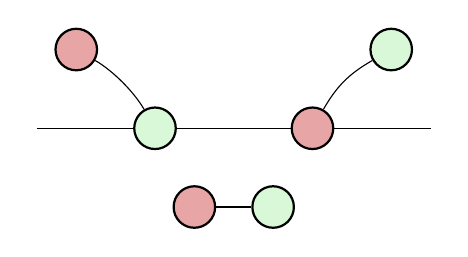
\begin{tikzpicture}
            \node [style=rn] (2) at (0, -1) {};
            \node [style=gn] (5) at (1, -1) {};
            \node [style=none] (6) at (-2, 0) {};
            \node [style=none] (7) at (3, 0) {};
            \node [style=gn] (8) at (-0.5, 0) {};
            \node [style=rn] (9) at (1.5, 0) {};
            \node [style=rn] (10) at (-1.5, 1) {};
            \node [style=gn] (11) at (2.5, 1) {};
            \draw (2) to (5);
            \draw (6.center) to (8);
            \draw (8) to (9);
            \draw (9) to (7.center);
            \draw [bend left=15, looseness=0.75] (10) to (8);
            \draw [bend right=15] (11) to (9);
    \end{tikzpicture}    
\end{center}
Diagram preuredimo
\begin{center}
    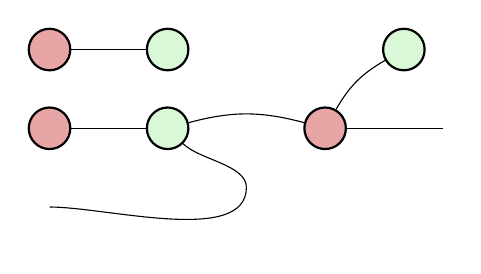
\begin{tikzpicture}
            \node [style=rn] (2) at (-2, 1) {};
            \node [style=gn] (5) at (-0.5, 1) {};
            \node [style=none] (6) at (0.5, -0.75) {};
            \node [style=none] (7) at (3, 0) {};
            \node [style=gn] (8) at (-0.5, 0) {};
            \node [style=rn] (9) at (1.5, 0) {};
            \node [style=rn] (10) at (-2, 0) {};
            \node [style=gn] (11) at (2.5, 1) {};
            \node [style=none] (12) at (-2, -1) {};
            \draw (2) to (5);
            \draw [in=-45, out=90, looseness=0.75] (6.center) to (8);
            \draw [bend left=15] (8) to (9);
            \draw (9) to (7.center);
            \draw (10) to (8);
            \draw [bend right=15] (11) to (9);
            \draw [in=-90, out=0, looseness=0.75] (12.center) to (6.center);
    \end{tikzpicture}
\end{center}
in uporabimo pravilo kopiranja \ref{kopiranje}.
\begin{center}
    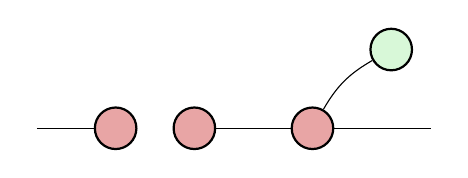
\begin{tikzpicture}
            \node [style=none] (7) at (3, 0) {};
            \node [style=rn] (9) at (1.5, 0) {};
            \node [style=gn] (11) at (2.5, 1) {};
            \node [style=none] (12) at (-2, 0) {};
            \node [style=rn] (13) at (-1, 0) {};
            \node [style=rn] (14) at (0, 0) {};
            \draw (9) to (7.center);
            \draw [bend right=15] (11) to (9);
            \draw (12.center) to (13);
            \draw (14) to (9);
    \end{tikzpicture}    
\end{center}
Kar lahko združimo \ref{zdruzitev} in poenostavimo z izbrisom identitet \ref{identiteta}, kar dokaže lastnost.
\begin{center}
    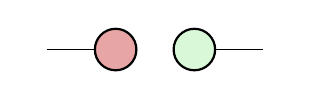
\begin{tikzpicture}
        \node [style=none] (0) at (0,0) {};
        \node [style=rn] (1) at (1,0) {};
        \node [style=gn] (2) at (2,0) {};
        \node [style=none] (3) at (3,0) {};
        \draw (0) to (1);
        \draw (2) to (3);
    \end{tikzpicture}
\end{center}
\subsection{Lastnosti}
Da upravičimo uporabo ZX-računa želimo nekaj dobrih lastnosti. Že prej smo omenili polnost jezika, obstaja pa še nekaj ostalih temelnjih lastnosti, katerih si želimo. Najbolj osnovna lastnost je pravilnost.
\subsubsection{Pravilnost}
\begin{izrek}[Pravilnost]
    Če lahko diagram \(D_1:n\to m\) prepišemo v \(D_2:n\to m\) z uporabo aksiomov ZX-računa, potem \(\interpret{D_1} = \interpret{D_2}\).
\end{izrek}
Ta izrek enostavno preverimo tako, da razpišemo leve in desne strani enakosti podanih v aksiomih ter vidimo, da se ujemajo \cite[izrek 2.16]{Coecke_2011}. Bolj težavna je le topološka ekvivalenca grafov (specifično to, da lahko vhode in izhode vozlišč menjamo), saj ne moremo opazovati le enega elementa v izolaciji, pač pa interakcije med različnimi elementi. Še vedno bi to lahko dokazali z razpisovanjem, bolj pogosto pa se uporabi to, da model prevedemo v jezik kategorij \cite[izrek 4.24]{Coecke_2011}.

Tukaj velja še omeniti skalarne grafe. To so grafi brez vhodov in izhodov, prisotni v mnogih aksiomih, na primer pravilu kopiranja \ref{kopiranje}. Mnogi pristopi v aksiomih izpustijo skalarne grafe, vendar v tem primeru pravilnost ne velja. To sicer nima velikega praktičnega pomena, saj pravilnost še vedno velja do skalarja natančno, zaradi unitarnosti kvantnih preslikav pa ne izgubimo veliko informacij zaradi skalarjev. V tem primeru delamo z ekvivalenčnimi razredi matrik.
\subsubsection{Polnost}
\begin{izrek}[Polnost]
    Če imamo dva diagrama \(D_1:n\to m\) in \(D_2:n\to m\), za katera velja \(\interpret{D_1} = \interpret{D_2}\), potem lahko \(D_1\) pretvorimo v \(D_2\) (ali obratno) z uporabo aksiomov.
\end{izrek}
Že od samega začetka uvedbe ZX-računa je bila polnost najbolj iskana lastnost jezika. Dovoli namreč, da lahko vsako lastnost, ki drži v Diracovem formalizmu, dokažemo tudi v ZX računu. Prvotne izbire aksiomov niso bile polne, kar je omejilo ekspresivnost jezika in možnost njegove uporabe. Večina formalizacij je potrebovala nekakšen nelinearen aksiom, pri nas pa za to poskrbi aksiom Eulerjevih kotov \ref{euler}. Že pri zgodnjih rezultatih so sumili, da je podoben aksiom potreben \cite{Schr_der_de_Witt_2014}, vendar ni bilo znano, ali je zadosten. Kasneje pa so dokazali, da je bila to edina večja prepreka, dokaz polnosti pa je potekal preko podobnega grafičnega jezika, ZW-račun, za katerega je bila polnost že znana \cite{kangfengng}.

\subsubsection{Univerzalnost}
\begin{izrek}[Univerzalnost]
    Za poljubno linearno preslikavo kubitov \(A:\C^{2^n}\to \C^{2^m}\), ki preslika \(n\) kubitov v \(m\) kubitov, obstaja ZX diagram \(D:n\to m\) za katerega \(\interpret{D}=A\)
\end{izrek}
\proof
Vemo, da lahko poljubno unitarno preslikavo \(n\) kubitov napišemo z uporabo cNOT vrat ter eno kubitnih unitarnih preslikav \cite[Izrek 5.26]{mathforqm}. Če to naredimo, je potreben le opis kako prevesti cNOT vrata v ZX račun in kako prevesti splošno enokubitno unitarno preslikavo v ZX račun. Vemo, da cNOT vratom pripada matrika
\begin{align*}
    \begin{bmatrix}
        1&0&0&0\\
        0&1&0&0\\
        0&0&0&1\\
        0&0&1&0
    \end{bmatrix}.
\end{align*}
Interpretacija diagrama
\begin{center}
    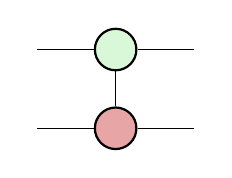
\begin{tikzpicture}
            \node [style=gn] (0) at (0, 1) {};
            \node [style=rn] (1) at (0, 0) {};
            \node [style=none] (2) at (-1, 1) {};
            \node [style=none] (3) at (-1, 0) {};
            \node [style=none] (4) at (1, 1) {};
            \node [style=none] (5) at (1, 0) {};
            \draw (2.center) to (0);
            \draw (0) to (4.center);
            \draw (3.center) to (1);
            \draw (1) to (5.center);
            \draw (0) to (1);
    \end{tikzpicture}  
\end{center}
pa je ravno ta matrika. Poljubno unitarno preslikavo enega kubita pa lahko napišemo kot kompozitum Eulerjevih kotov \cite[Izrek 5.11]{mathforqm}. Pajki sami pa po definiciji ustrezajo rotacijam okoli X in Z osi. Torej lahko poljubno unitarno preslikavo napišemo kot
\begin{center}
    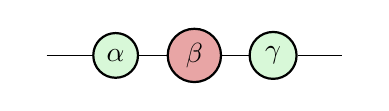
\begin{tikzpicture}
        \node [style=none] (0) at (0,0) {};
        \node [style=gn] (1) at (1,0) {\(\alpha\)};
        \node [style=rn] (2) at (2,0) {\(\beta\)};
        \node [style=gn] (3) at (3,0) {\(\gamma\)};
        \node [style=none] (4) at (4,0) {};
        \draw (0) to (1) to (2) to (3) to (4);
    \end{tikzpicture}.
\end{center}
Sedaj imamo univerzalnost za preslikave \(n\) kubitov v \(n\) kubitov. Kvantna stanja dobimo kot sliko takšne preslikave, za poljubno željeno kvantno stanje \(n+m\) kubitov po univerzalnosti obstaja ZX diagram, ki vhod \(n+m\) zelenih pajkov preslika v to stanje. Diagram, ki to predstavlja je \(n+m\) zelenih pajkov, ki vodijo v preostanek diagrama, ven iz diagrama pa vodi \(n+m\) povezav. Zaradi topološke ekvivalence grafov pa ni razlike med \(n+m\) izhodov ter \(n\) vhodov in \(m\) izhodov, saj lahko \(n\) izhodnih povezav prestavimo, da iz diagrama izhajajo na levo. Tako pa dobimo diagram, ki sprejme \(n\) kubitov, odda pa jih \(m\), predstavlja pa poljubno kvantno preslikavo, kar dokaže univerzalnost \cite[Izrek 2.18]{Coecke_2011}. \endproof
% NOTE še za n->m namesto n->n !!!

Izrek o univerzalnosti nam pove, da so diagrami dovolj ekspresivni in lahko opišejo poljubno transformacijo kubitov. Izrek o polnosti pa nam pove, da niso \emph{preveč} ekspresivni in bi lahko neko transformacijo opisali na več neekvivalentnih načinov. Če združimo izreka skupaj dobimo, da lahko vsako kvantno transformacijo napišemo na natanko en način, do pravil prepisovanja natančno.

\subsection{Drobci}
Pogosto omejimo faze, ki jih lahko uporabimo. Če v fazah pajkov dovolimo le večkratnike \(\frac\pi2\) imenujemo to Cliffordov drobec ali \(frac\pi2\) drobec. Če dovolimo \(\frac\pi4\) imenujemo to Clifford+T drobec.
\subsection{Kategorična slika}
\subsection{Dodatki}
\section{Kvantna mehanika z grafičnimi vezji}
\section{Poenostavjanje vezij}
\subsection{Quantomatic}
\section{Kvantni algoritmi in programiranje}
\subsection{Deutsch-Jozsov algoritem}
Najprej si definiramo nekaj pojmov.
\begin{definicija} Funkcija \(f:\{0,1\}^n\to \{0,1\}\) je konstantna, če \(\forall x\in\{0,1\}^n\sep f(x) = f(0,\ldots, 0)\).\end{definicija}
\begin{definicija}
    Funkcija \(f: \{0,1\}^n \to \{0,1\}\) je uravnotežena, če \(\exists S, U\subseteq \{0,1\}^n\) za katere \(\lvert S\rvert = \lvert U\rvert\) in \(f(S) = \{1\}, f(U) = \{0\}\)
\end{definicija}
Z drugimi besedami, funkcija je konstantna, če preslika vse argumente v isto vrednost in je uravnotežena, če preslika natanko polovico elementov v eno vrednost, drugo polovico pa v drugo.

Deutsch-Jozsov algoritemu podamo funkcijo \(f\) z zagotovilom, da je ali konstantna ali uravnotežena, ta nam pa v eni sami evaluaciji funkcije \(f\) odgovori katero izmed teh dveh opcij je.
\subsection{Kvantno iskanje}
Dano imamo funkcijo \(f: \{0,1\}^n\to \{0,1\}\) z zagotovilom, da se točno ena četrtina vhodov preslika v \(1\). Cilj je poiskati nek vhod \(x\in\{0,1\}^n\) pri katerem \(f(x) = 1\). S klasičnim algoritmom brez uporabe kvantne mehanike ugotovimo pravi odgovor z verjetnostjo \(0.25\), v najslabšem primeru pa moremo preveriti kar tri četrtine vhodov! Kvantni algoritm nam vedno da odgovor v eni evaluaciji funkcije.
\subsection{Računanje preko meritev}


\section*{Slovar strokovnih izrazov}

\geslo{Hilbert space}{Hilbertov prostor}
\geslo{observable}{opazljivka}
\geslo{state}{stanje}
\geslo{qubit}{kubit}
\geslo{balanced function}{uravnotežena funkcija}


\printbibliography
\end{document}

